%%
%% trouser.tex
%% 
%% Made by Alex Nelson
%% Login   <alex@black-cherry>
%% 
%% Started on  Mon Aug 24 10:35:19 2009 Alex Nelson
%% Last update Mon Aug 24 10:35:19 2009 Alex Nelson
%%

\begin{wrapfigure}{r}{0.55\textwidth}
  \begin{center}
    \includegraphics[width=0.48\textwidth]{img/img0.eps}
  \end{center}
  \caption{\footnotesize {Trouser Diagram}}
\end{wrapfigure}
We first set up the trousers diagram, as doodled on the right. It
basically is a cobordism from one circle to two (disjoint)
circles. The boundaries (well, the notion of a circle to be more
precise) consist of 1 edge and 1 vertex (each). So $e_{i}$ is the
edge that starts and ends at $v_{i}$ (where $i=1,2,3$). We have
two additional edges which connects the initial state (the
$e_{1}$, $v_{1}$ circle) to the terminal state (the $e_{2}$,
$e_{3}$ circles). These edges define the trousers diagram. We are
interested in calculating the various algebraic quantities which
will be used in the homological calculations, which we use
motivated by discrete differential geometry.

\begin{wrapfigure}{l}{0.55\textwidth}
  \begin{center}
    \includegraphics[width=0.55\textwidth]{img/img1.eps}
  \end{center}
  \caption{Initial/terminal states highlighted.}
\end{wrapfigure}
To begin setting up a chain to describe the initial and terminal
states (doodled on the left in red and blue, respectively), we
should consider the number of edges and vertices.
We see that we don't need to consider anything ``higher'' than
vertices and edges since there are no $p$-cells. Let $r_{v}$ be
the number of red vertices, $r_{e}$ be the number of red
edges. We see that the chain describing the initial state is
$0 \leftarrow C_{0}\leftarrow C_{1}$
where $C_{0}\cong\mathbb{Z}^{r_{v}}$ and
$C_{1}\cong\mathbb{Z}^{r_{e}}$ are the free groups generated by
the vertices and edges in the initial state (respectively). 
\clearpage

We thus have our chain describing our initial state be:
\begin{equation}%\label{eq:}
0 \leftarrow \mathbb{Z}\leftarrow \mathbb{Z}
\end{equation}
Now, we would like a corresponding chain describing the final
state. We see, similarly, that the chain would be 
\begin{equation}%\label{eq:}
0\leftarrow C_{1}' \leftarrow C_{2}'
\end{equation}
where $C_{1}'\cong\mathbb{Z}^{b_{v}}$ and
$C_{2}'\cong\mathbb{Z}^{b_{e}}$, $b_{v}$ is the number of blue
vertices, $b_{e}$ is the number of blue edges. We see by
inspection that $b_{v}=2$ and $b_{e}=2$, thus the chain
describing the final state is
\begin{equation}%\label{eq:}
0\leftarrow\mathbb{Z}^{2}\leftarrow\mathbb{Z}^{2}.
\end{equation}
We would like a chain complex to describe the cobordism altogether.

The general scheme for the cobordism is
\begin{equation}\begin{CD}
\mathbb{Z}     @<<< \mathbb{Z} \\
@VVV                 @VVV\\
\mathcal{M}_{1} @<<< \mathcal{M}_{2} @<<< \mathcal{M}_{3} \\
@AAA                 @AAA\\
\mathbb{Z}^{2}  @<<< \mathbb{Z}^{2}
\end{CD}\end{equation}
where we are trying to find $\mathcal{M}_{1}$ which corresponds
to the free group generated by \emph{all} of the vertices in the
diagram, and $\mathcal{M}_{2}$ corresponds to the gree group
generated by \emph{all} of the edges in the diagram. 

\begin{wrapfigure}{r}{0.55\textwidth}
  \begin{center}
    \includegraphics[width=0.55\textwidth]{img/img2.eps}
  \caption{All vertices highlighted}
  \end{center}
\end{wrapfigure}
The
$\mathcal{M}_{3}$ corresponds to the free group generated by the
``skin'' of the cobordism, if we think of the edges as the
``bones'' the cobordism is somewhat analogous to a tent.
We see that there are only three edges in total in our
diagram. They are doodled on the left. The initial vertices are
in red, the terminal vertices are in blue. So we see that there
are 2+1=3 vertices telling us that
$\mathcal{M}_{1}\cong\mathbb{Z}^{3}$, which solves one part of
our problem. We are left with trying to deduce what the other
aspects of the chain complex could be.

We are worried about the edges, since we already deduced that
$\mathcal{M}_{3}\cong\mathbb{Z}$. There is only one ``skin'' to
the diagram. We can fill in the parts of the chain complex that
we know:
\begin{equation}\begin{CD}
\mathbb{Z}     @<<< \mathbb{Z} \\
@VVV                 @VVV\\
\mathbb{Z}^{3} @<<< \mathcal{M}_{2} @<<< \mathbb{Z} \\
@AAA                 @AAA\\
\mathbb{Z}^{2}  @<<< \mathbb{Z}^{2}
\end{CD}\end{equation}
We need to deduce what $\mathcal{M}_{2}$ is.

\begin{figure}[h]%{0.50\textwidth}
  \begin{center}
    \includegraphics[width=0.48\textwidth]{img/img3.eps}
  \end{center}
  \caption{All edges highlighted.}\label{fig:img3}
%  \end{center}
\end{figure}
Doodled above in figure \eqref{fig:img3} is the diagram with \emph{all} of the edges
highlighted. The initial edge is in red, the terminal edge is in
blue, and the intermediate edges are in purple. We see that there
is a total of 1+2+2=5 edges, which allows us to deduce that
$\mathcal{M}_{2}\cong\mathbb{Z}^{5}$. This is the last part of
the computation of the chain complex, the rest of the calculation
for this particular cobordism is strictly manipulation via the
functor \textbf{nChain}$\to$\textbf{Hilb}. (This won't require
too much algebraic manipulation since we are working with
regular, old fashioned electromagnetism, so we are concerned with
assigning information from U(1) to edges; the compactness of U(1)
simplifies life significantly.) To summarize, the chain
calculation is finished with
\begin{equation}\begin{CD}
\mathbb{Z}     @<<< \mathbb{Z} \\
@VVV                 @VVV\\
\mathbb{Z}^{3} @<<< \mathbb{Z}^{5} @<<< \mathbb{Z} \\
@AAA                 @AAA\\
\mathbb{Z}^{2}  @<<< \mathbb{Z}^{2}
\end{CD}\end{equation}

Let 
\begin{equation}%\label{eq:}
Z:\mathbf{nChain}\to\mathbf{Hilb}
\end{equation}
be the chain field theory describing regular, old-school
electromagnetism (i.e. the connections are defined on the edges,
the gauge is U(1), etc.). The time evolution of our doodle is
described by the morphism
\begin{equation}%\label{eq:}
Z(\mathbb{Z})\to Z(\mathbb{Z}^{2}).
\end{equation}
With gauge systems, we typically find the physically meaningful
states by taking the orbit of the gauge group modulo the
stabilizer. Similarly, the physically meaningful states would be
\begin{equation}%\label{eq:}
Z(C)\cong L^{2}\left(\frac{\mathcal{A}(C)}{\mathcal{G}(C)}\right)
\end{equation}
where $\mathcal{A}(C):=C^{p}=$ group of p-connections, and
$\mathcal{G}(C):=C^{p-1}=$ gauge group,
$C^{p}:=\hom(C_{p},U(1))$. For those of us interested in
old-school electromagnetism this is 1-connections. We see that
for compact groups we don't have to mod out by the gauge
transformations, so we integrate over the connections on the
manifold.

\begin{rmk}
Remember that connections are elements of
$\hom(\mathbb{Z}^{X_{p}},U(1))$. That is, functions assigning to
elements of the free group generated by the p-cells $X_{p}$ data
from our group U(1).
\end{rmk}

We end up with
\begin{equation}%\label{}
Z(C)\cong L^{2}\left[\hom\Big(\mathbb{Z},U(1)\Big)\right]
\end{equation}
since there is only one edge in the initial state.

\begin{prop}%\label{prop:}
We have the following isomorphism
\begin{equation}%\label{eq:}
\hom(\mathbb{Z},U(1))\cong U(1).
\end{equation}
\end{prop}
\begin{proof}
We see that for $\varphi\in\hom(\mathbb{Z},U(1))$ that
\begin{equation}%\label{eq:}
\varphi(1)=\alpha\quad\Rightarrow\quad \varphi(n)=a^{n}
\end{equation}
since $n=1+\cdots+1$ which uses the law of composition in
$\mathbb{Z}$ as a free group. This is preserved by a homomorphism
$\varphi$ and becomes multiplication (the law of composition) in
the group U(1). Since the choice of $a=\exp(i\theta)$ is
arbitrary (for some $\theta\in[0,2\pi)$), we can choose a
  different $\varphi$ for each $\theta$ mapping all of
  $\mathbb{Z}$ to all of U(1).
\end{proof}
\begin{comment}
\begin{proof}
The proof is more or less roundabout. We know that an element of
$U(1)$ looks like $\exp(i\theta)$ for some
$\theta\in\mathbb{R}$. We know we can construct $\mathbb{R}$ from
$\mathbb{Q}$, and we can construct $\mathbb{Q}$ from
$\mathbb{Z}$. So we consider a family of homomorphisms
\begin{equation}%\label{eq:}
\phi_{m}(n)=\exp(in/m)\in\hom(\mathbb{Z},U(1))
\end{equation}
which really gives us two degrees of freedom to play around with:
$m$ and $n$. This is precisely just $(n/m)\in\mathbb{Q}$. This
allows us to embed
\begin{equation}%\label{eq:}
\hom(\mathbb{Q},U(1))\subseteq\hom(\mathbb{Z},U(1))
\end{equation}
We can construct from $\mathbb{Q}$ the reals, which allows us to
have an isomorphism
$\hom(\mathbb{Q},U(1))\cong\hom(\mathbb{R},U(1))$ but this is
precisely $U(1)$. Thus by our deduction, there is an
isomorphism from $\hom(\mathbb{R},U(1))$ to a subset of
$\hom(\mathbb{Z},U(1))$, and there is the obvious isomorphism
$\hom(\mathbb{R},U(1))\cong U(1)$ which proves the hypothesis.
\end{proof}
\end{comment}

By our proposition, we have that
\begin{equation}%\label{eq:}
Z(\mathbb{Z})\cong L^{2}(U(1)).
\end{equation}
Similarly, we have for the target
\begin{equation}%\label{eq:}
Z(\mathbb{Z}^{2})\cong L^{2}\Big(U(1)\otimes U(1)\Big).
\end{equation}
Thus our cobordism give the time evolution by the functor
\begin{equation}%\label{eq:}
Z(M): L^{2}(U(1))\to L^{2}\Big(U(1)\otimes U(1)\Big).
\end{equation}
The question we want to answer is: \emph{how exactly does it
  work?}

The strategy is that we'll consider the object $Z(M)$ as a
mathematical operator, and we recall from linear algebra to
compute the entries of an operator we have to compute how it acts
on basis elements. 

First we need to pick some elements of $L^{2}(U(1))$ and
$L^{2}(U(1))^{\otimes 2}$. Remember that we are working
with connections, i.e. functions from $C_{p}$ to $U(1)$. So we
should choose for $L^{2}(U(1))$ functions of the form
\begin{equation}%\label{eq:}
\psi(A) = \exp(ikA).
\end{equation}
Similarly for $L^{2}(U(1))^{\otimes 2}$ we have a
``tensor product'' of two such functions yielding one that looks
like
\begin{equation}%\label{eq:}
\phi(A_{1},A_{2}) = \exp(ikA_{1})\exp(ikA_{2}).
\end{equation}
We will use such functions to figure out the components of the
operator in question.

\begin{prop}\label{prop:fourierExpansionThetaFunction}
We have by Fourier expansion:
\begin{equation}%\label{eq:}
\sum_{n\in\mathbb{Z}}\exp\left(\frac{-1}{2e^{2}V}(A+2n\pi)^{2}\right)
= \sum_{n\in\mathbb{Z}}\exp\left(\frac{-e^{2}Vn^{2}}{2}\right)e^{inA}
\end{equation}
(up to some constant coefficient).
\end{prop}

\begin{figure}[t]
\includegraphics{img/img4.eps}
\caption{The manifold with orientation picked arbitrarily. The
  curvature calculations depend on the parts of the figure
  colored in. Red contributions are positive, blue contributions
  are negative}\label{fig:img4}
\end{figure}

Well, we find by eq (16) of \cite{Wise:2006kg} that
\begin{equation}%\label{eq:}
\<{\color{red}\!\!\overbracket[0.25pt]{~\phi~}^{\mathrlap{\;\;\;\;\;\;\;\;\in L^{2}(U(1))^{\otimes 2}}}\!\!},Z(M){\color{blue}\!\underbracket[0.25pt]{\,\,\psi~}_{\mathrlap{\;\;\;\;\;\;\in L^{2}(U(1))}}\!\!}\> =
\int_{{\substack{\text{connections}\\\text{on $\mathcal{M}$}}}}\overline{\phi(A|_{S'})}\psi(A|_{S}) e^{-S(A)}\mathcal{D}A
\end{equation}
where $S(A)$ is the action. This allows us to compute entries in
$Z(M)$, kind of like how we compute entries in the $S$-matrix. We
see in section 7 (et seq) of \cite{Wise:2006kg} that the path integral
should consider
\begin{equation}%\label{eq:}
\begin{pmatrix}p$-connections$\\
$on$\ \mathcal{M}\end{pmatrix}
=U(1)^{X_{p}}.
\end{equation}
For us $p=1$ and $|X_{1}|=5$, so the measure $\mathcal{D}A$ in
our case becomes
\begin{equation}%\label{eq:}
\mathcal{D}A = \frac{dA_{1}}{2\pi}\frac{dA_{2}}{2\pi}\frac{dA_{3}}{2\pi}\frac{dA_{4}}{2\pi}\frac{dA_{5}}{2\pi}
\end{equation}
To calculate the action, we need to pick an orientation for the
manifold. We do this in figure \ref{fig:img4}, and we calculate
the curvature of the entire manifold to be:
\begin{equation}%\label{eq:}
\begin{split}
F =&
A(e_{3})-A(e_{4})+A(e_{1})+A(e_{4})-A(e_{5})+A(e_{2})+A(e_{5}) \\
=& A(e_{3})+A(e_{1})+A(e_{2})
\end{split}
\end{equation}
We end up with the integrand being
\begin{equation}%\label{eq:}
\overline{\phi(A|_{S'})}\psi(A|_{S}) e^{-S(A)}=e^{-ikA_{1}}e^{-ikA_{2}}e^{ikA_{3}}\sum_{n\in\mathbb{Z}}\exp\left(\frac{-h}{2e^{2}}(F+2\pi n)^{2}\right)
\end{equation}
where we sum over $\mathbb{Z}^{X_{p+1}}=\mathbb{Z}^{1}$. We can
now rewrite our integral to be
\begin{equation}%\label{eq:}
\begin{split}
\<\phi,Z(M)\psi\> &=
\iint^{2\pi}_{0}\frac{dA_{4}}{2\pi}\frac{dA_{5}}{2\pi}
\iiint^{2\pi}_{0}e^{-ikA_{1}}e^{-ikA_{2}}e^{ikA_{3}}\sum_{n\in\mathbb{Z}}\exp\left(\frac{-h}{2e^{2}}(F+2\pi n)^{2}\right)\frac{dA_{1}}{2\pi}\frac{dA_{2}}{2\pi}\frac{dA_{3}}{2\pi}\\
&= \iiint^{2\pi}_{0}e^{-ikA_{1}}e^{-ikA_{2}}e^{ikA_{3}}\sum_{n\in\mathbb{Z}}\exp\left(\frac{-h}{2e^{2}}(F+2\pi n)^{2}\right)\frac{dA_{1}}{2\pi}\frac{dA_{2}}{2\pi}\frac{dA_{3}}{2\pi}
\end{split}
\end{equation}
The factor $\iint dA_{4}dA_{5}$ end up contributing a factor
of 1. 

By proposition \eqref{prop:fourierExpansionThetaFunction} we see
that (up to a constant) we can simplify our expression to a
friendler one:
\begin{equation}%\label{eq:}
\<\phi,Z(M)\psi\> = \iiint^{2\pi}_{0}e^{-ikA_{1}}e^{-ikA_{2}}e^{ikA_{3}}\sum_{n\in\mathbb{Z}}\exp\left(\frac{-e^{2}Vn^{2}}{2}\right)\exp(inF)\frac{dA_{1}}{2\pi}\frac{dA_{2}}{2\pi}\frac{dA_{3}}{2\pi}.
\end{equation}
We just need to plug in our expression for the curvature $F$ and
manipulate it a little to get the solution. Recall first that the
kronecker delta is defined by
\begin{equation}%\label{eq:}
\delta_{x,n} = \int^{2\pi}_{0} e^{i(x-n)\theta}d\theta
\end{equation}
this will come in handy in a few moments.

By rearranging terms and expanding out the expression for the
curvature, we end up with
%\begin{subequations}
\begin{align*}
\<\phi,Z(M)\psi\> &= \iiint^{2\pi}_{0}e^{-ikA_{1}}e^{-ikA_{2}}e^{ikA_{3}}\sum_{n\in\mathbb{Z}}\exp\left(\frac{-e^{2}Vn^{2}}{2}\right)\exp(inF)\frac{dA_{1}}{2\pi}\frac{dA_{2}}{2\pi}\frac{dA_{3}}{2\pi}\\
&=\iint^{2\pi}_{0}e^{-ikA_{1}}e^{-ikA_{2}}\sum_{n\in\mathbb{Z}}\exp\left(\frac{-e^{2}Vn^{2}}{2}\right)\exp(inA_{1}+inA_{2})\frac{dA_{1}}{2\pi}\frac{dA_{2}}{2\pi}\color{red}{\underbracket[0.25pt]{\int^{2\pi}_{0}e^{i(n+k)A_{3}}\frac{dA_{3}}{2\pi}}_{\text{not quite right...}}}
\end{align*}
%\end{subequations}
Note that the term in red on that last line is not quite
right. The only explanation I could find is that I botched the
curvature calculation, it should be
\begin{equation}%\label{eq:}
F = A_{1}+A_{2}-A_{3}
\end{equation}
which then produces the correct expression, yielding for our calculations
\begin{equation}%\label{eq:}
\<\phi,Z(M)\psi\> = \iint^{2\pi}_{0}e^{-ikA_{1}}e^{-ikA_{2}}\sum_{n\in\mathbb{Z}}\exp\left(\frac{-e^{2}Vn^{2}}{2}\right)\exp(inA_{1}+inA_{2})\frac{dA_{1}}{2\pi}\frac{dA_{2}}{2\pi}\underbracket[0.25pt]{\int^{2\pi}_{0}e^{i(n-k)A_{3}}\frac{dA_{3}}{2\pi}}_{\delta_{k,n}}
\end{equation}
It allows us to reduce this to (by plugging  in the Kronecker
delta):
\begin{equation}%\label{eq:}
\<\phi,Z(M)\psi\> =
\iint^{2\pi}_{0}e^{-ikA_{1}}e^{-ikA_{2}}\underbracket[0.25pt]{\left[\sum_{n\in\mathbb{Z}}\exp\left(\frac{-e^{2}Vn^{2}}{2}\right)\exp(inA_{1}+inA_{2})\delta_{n,k}\right]}_{\text{identify as }Z(M)|\psi\>}\frac{dA_{1}}{2\pi}\frac{dA_{2}}{2\pi}
\end{equation}
The bracketed factor is identified with how the basis vector
$\exp(ikA_{3})$ behaves when acted on by the operator $Z(M)$. We
can simplify things to summarize it thus:
\begin{equation}%\label{eq:}
Z(M):e^{ikA_{3}}\mapsto \exp\left(\frac{-e^{2}Vk^{2}}{2}\right)\exp(ikA_{1}+ikA_{2})
\end{equation}
which is precisely the desired result.
